\documentclass[12pt, a4paper]{article}
\usepackage{graphicx} %bruk grafikk pakke
\graphicspath{PreSnooze/}
\begin{document}



\title{PreSnooze} 
\author{Kjetil Nordpoll Vatsøy}
\date{Aug 2024}

\maketitle

\pagebreak

\begin{figure}[h]
\centering
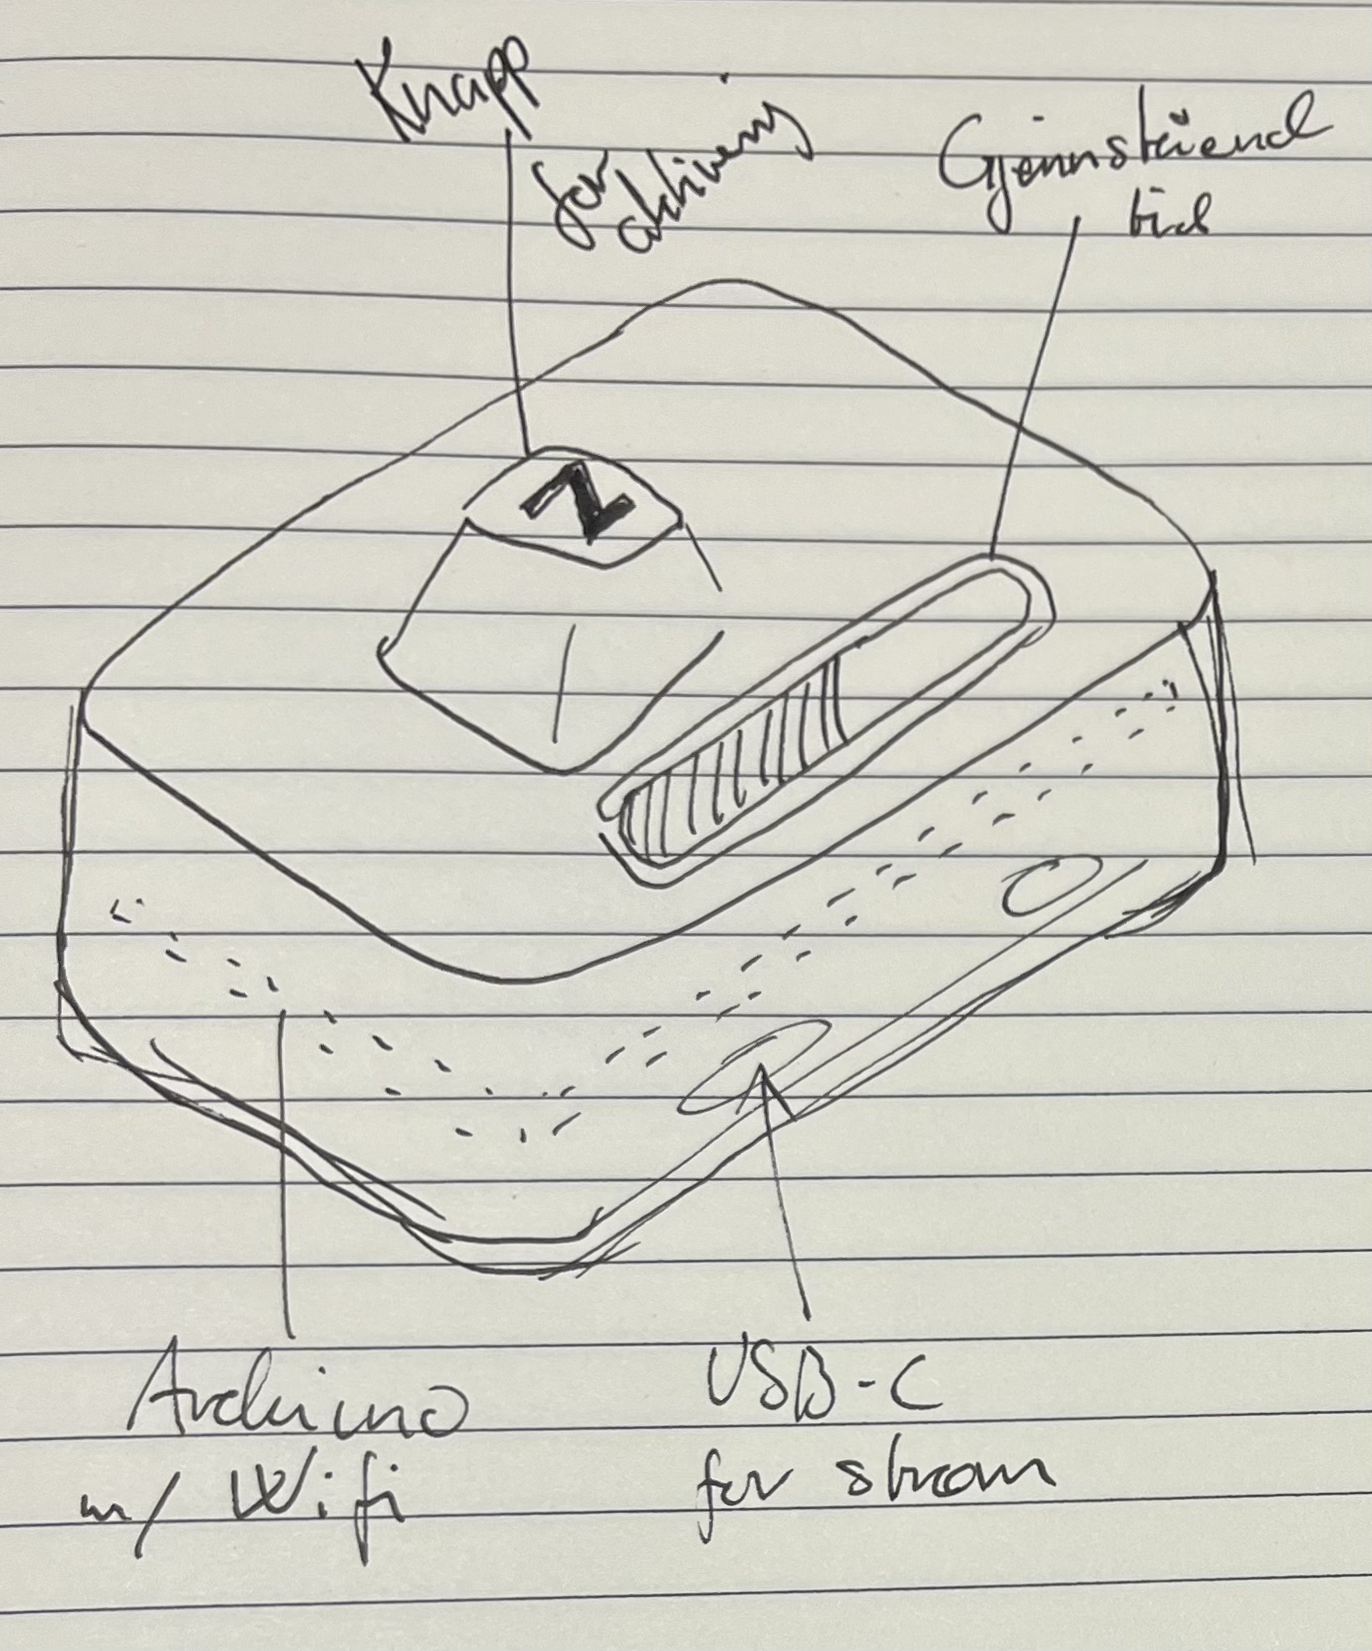
\includegraphics[width=0.75\textwidth]{IMG_2505.png}
\caption{Frist draft}
\end{figure}   

\begin{abstract}
Målet med PreSnooze er å løse problemet med for lite søvn i løpet av en natt. 
Dette gjøres ved at PreSnooze ikke alarmerer ved bestemt tid, men kalkulerer tidspunkt for alarmen. For eksempel tidspunket en trykker på knappen pluss 8 timer eller x antall søvnsykluser.
\end{abstract}

\pagebreak





\section*{Funksjoner}

\subsection {Hovedfunksjon:}
\begin{itemize}
    \item Setter alarm til x-antall søvnsykluser eller en bestemt tid
\end{itemize}


\subsection {Interface: }
\begin{itemize}
    \item Knapp / Riste / Klemme / Slider
\end{itemize}


\subsection {Aktuator:}
\begin{itemize}
    \item Alarm på telefonen / lyd / lys / bevegelse
\end{itemize}


\subsection {Strøm: }
\begin{itemize}
    \item Batterie / indusert strøm/ powersupply
\end{itemize}



\subsection {Tilleggsfunksjoner: }
\begin{itemize}
    \item Søvn i forskjellig lengde: 
    \item lur/lang lur/søvn
    \item integrasjon kalender
    \item 
\end{itemize}



\subsection {Fysiske egenskaper: }
\begin{itemize}
    \item Nattbordvennlig - 100x100x150
\end{itemize}


\subsection {Materiale:}
\begin{itemize}
    \item Tre er organisk
    \item 3d-print kan formes
    \item Lett å skru i plast
    \item Insterts for skruer i tre
\end{itemize}

\subsection {Compjuting:}
\begin{itemize}
    \item Input
2 Digital
1 Analog
    \item Output
3 analog
1 digital
    \item Wifi/Blåtann
\end{itemize}


\subsection {Fancy ideer: }
\begin{itemize}
    \item Hår
\end{itemize}


\end{document}